\chapter{適用例}\label{cha:Indication}
% 本章では、本研究で作成したモータ特性表自動生成ツールが正しく動作することを検証するため、以下の同じ能力である2種類のModelicaモデルのシミュレーション結果のcsvファイルを適用する。
本章では、本研究で作成したモータ特性表自動生成ツールが正しく動作することを確認する。
適用例として、ブラシ付きDCモータのModelicaモデルと、
ブラシ付きDCモータのModelicaモデルをサブシステムとするモデルの2つが出力するcsvファイルを適用例として用いる。
また、2つのモータの性能は同じである。
正しく動作しているか確認するために、以下の2つの点に着目する。
% 以下に示す2種類のModelicaモデルのシミュレーション結果のcsvファイルを適用例として用いる。
% 以下のモータは、性能は同じである。
% \begin{itemize}
%     \item ブラシ付きDCモータのModelicaモデル
%     \item ブラシ付きDCモータのModelicaモデルをサブシステムとするモデル
% \end{itemize}

% 2つのモデルのパラメータ設定を以下に示す。
% \begin{itemize}
%     \item 電源部品 ・・・ 9 V
%     \item 抵抗部品 ・・・ 1.78 $\Omega$
%     \item インダクタ部品 ・・・ 0.0000735 H
%     \item 起電力部品 ・・・ 0.010400000000000001 $mN \cdot m$
%     \item 慣性部品 ・・・ 0.00371135959 $\mathrm{kg\cdot m^2}$
% \end{itemize}
% 具体的には、以下の2つの項目を確認する。

\begin{enumerate}
    \item 生成したモータ特性表の各要素の値が、正しい値になっていること
    \item 2つのモデルから生成したモータ特性表の各要素が、同値になっていること
\end{enumerate}


\section{ブラシ付きDCモータのModelicaモデル}
\begin{figure}[t]
	\centering
	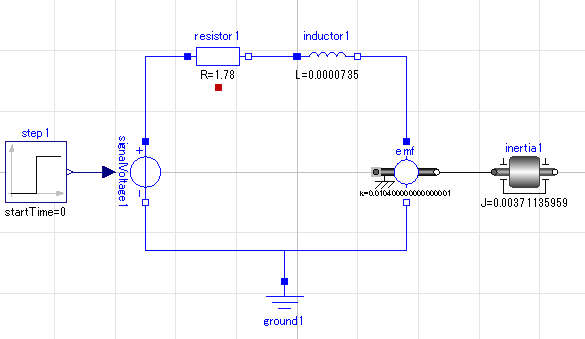
\includegraphics[width=10cm]{./Image/tekiyou_tanntai.png}
	\caption{適用するブラシ付きDCモータのModelicaモデル}
	\label{fig:tekiyou_tanntai}
\end{figure}

\begin{figure}[t]
	\centering
	\fbox{
    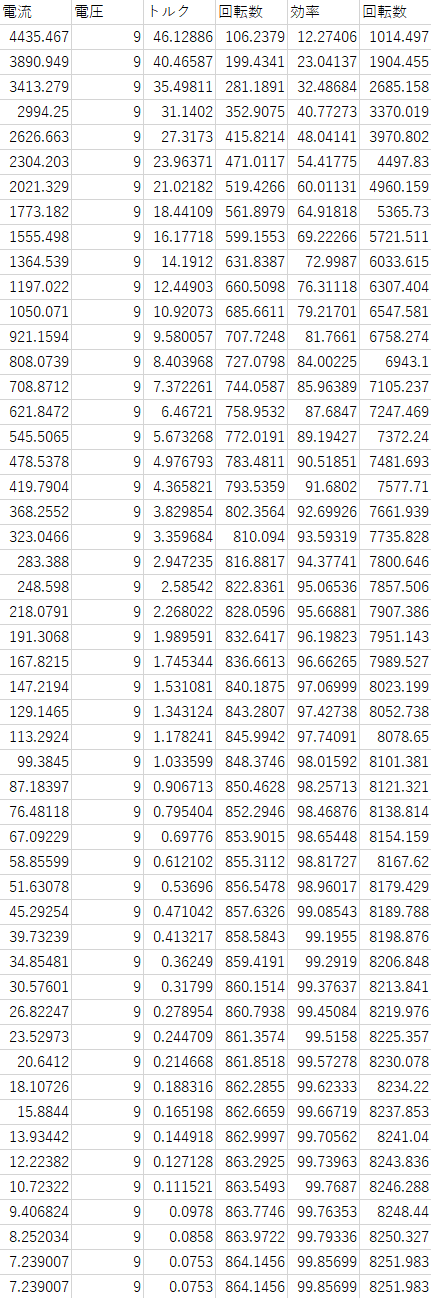
\includegraphics[width=13cm]{./Image/kakunin_csv.png}
    }
	\caption{図\ref{fig:tekiyou_tanntai}のシミュレーション結果であるcsvファイルの一部}
	\label{fig:tekiyou_csv}
\end{figure}

\begin{figure}[t]
	\centering
	\fbox{
	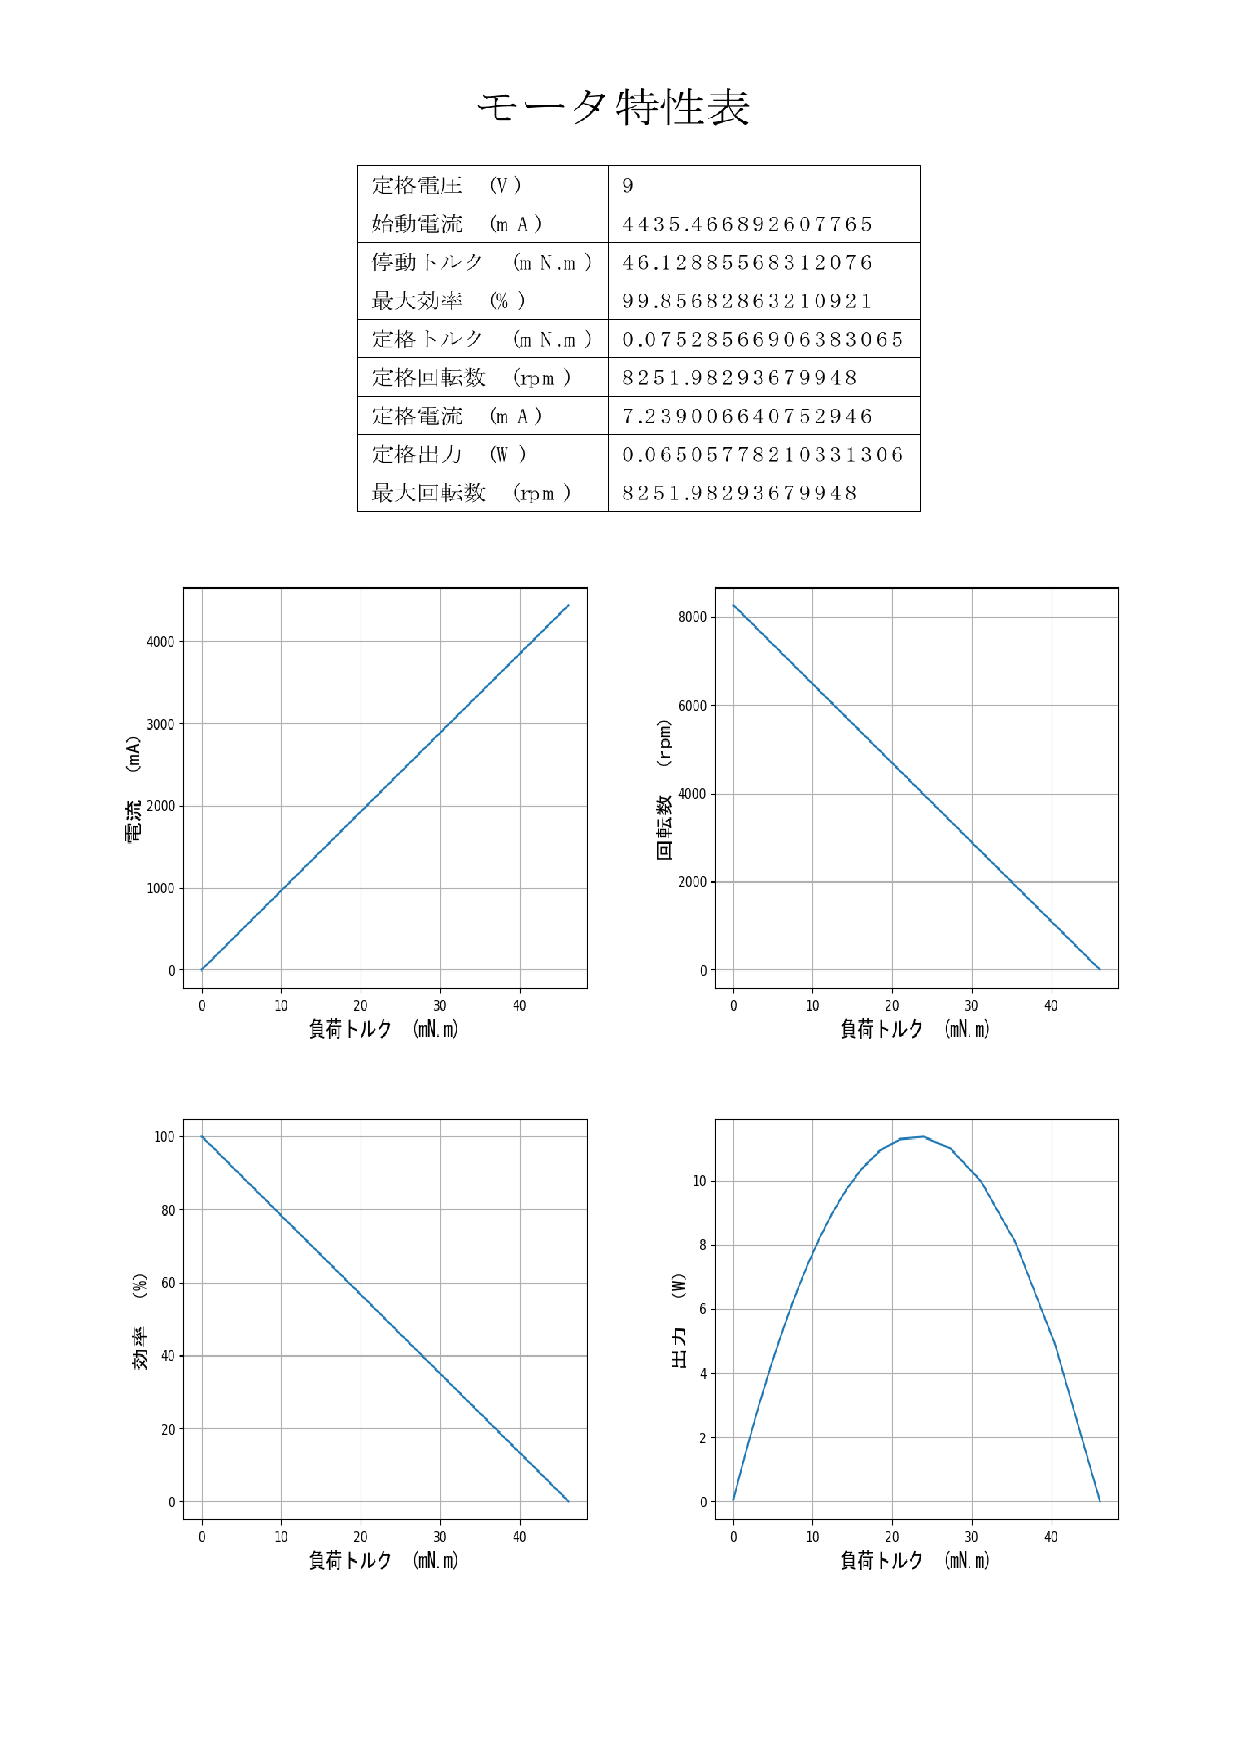
\includegraphics[width=16cm,pagebox=cropbox]{Image/characteristicTable_kakunin.pdf} 
	}
	\caption{適用例で生成したモータ特性表}
	\label{fig:tekiyou_mortoku}
\end{figure}

ブラシ付きDCモータのModelicaモデルをOpenModelicaで実行し、生成されたcsvファイルを、モータ特性表自動生成ツールに適用する。
適用例に用いるモデルを、図\ref{fig:tekiyou_tanntai}に示す。
また、図\ref{fig:tekiyou_tanntai}のシミュレーション結果であるcsvファイルを、図\ref{fig:tekiyou_csv}に示す。
図\ref{fig:tekiyou_csv}のcsvファイルをモータ特性表自動生成ツールに適用した結果、出力するモータ特性表を図\ref{fig:tekiyou_mortoku}に示す。

% \begin{figure}[t]
% 	\centering
% 	\fbox{
%     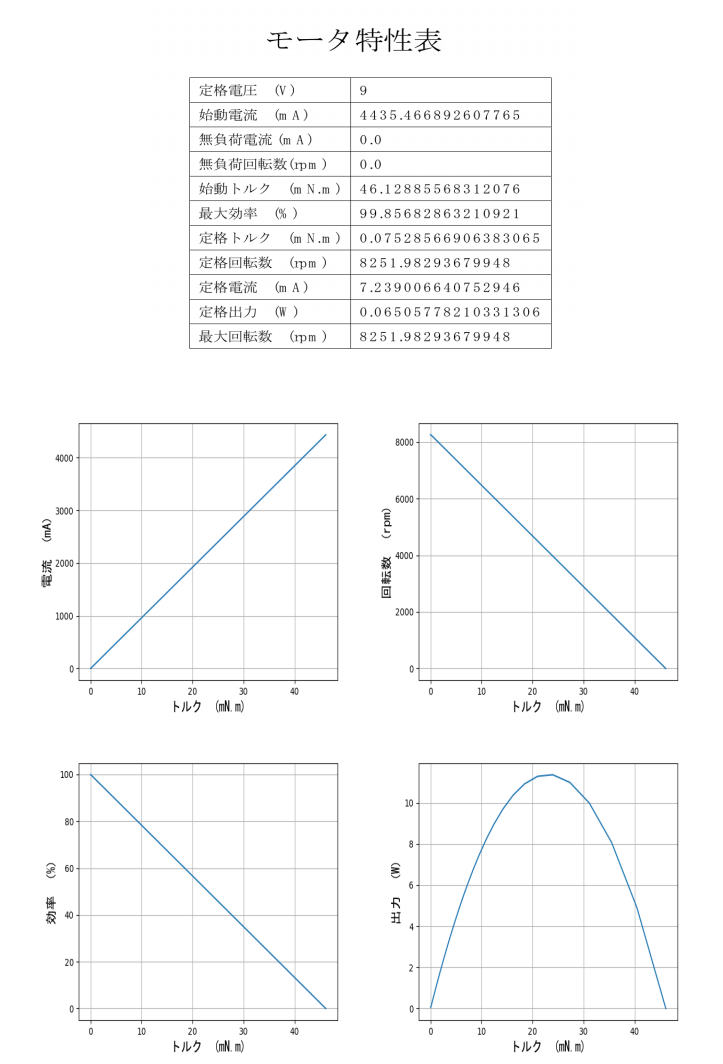
\includegraphics[width=14cm]{./Image/tekiyou_mortoku.png}
%     }
%     \caption{適用例で生成したモータ特性表}
% 	\label{fig:tekiyou_mortoku}
% \end{figure}
\begin{figure}[t]
	\centering
	\fbox{
    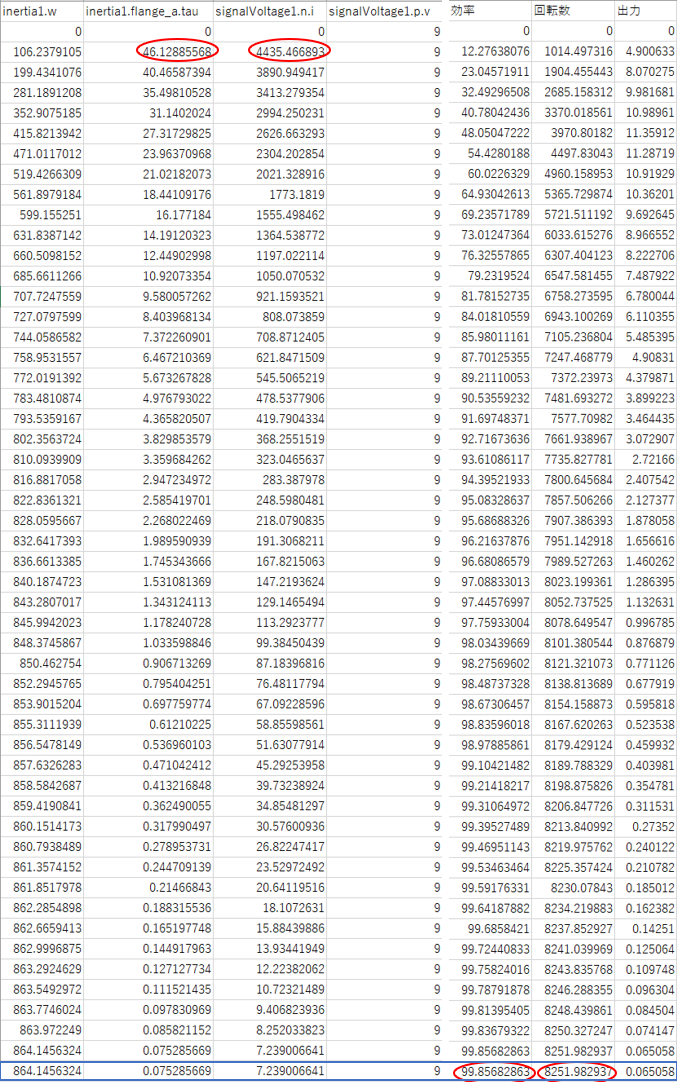
\includegraphics[width=13cm]{./Image/kakunin_saidai_mark.png}
    }
	\caption{図\ref{fig:tekiyou_tanntai}のシミュレーション結果であるcsvファイルの一部と効率と回転数と出力}
	\label{fig:tekiyou_csv_wakariyasui}
\end{figure}

\clearpage

\subsection{特性表の確認}
図\ref{fig:tekiyou_tanntai}のシミュレーション結果であるcsvファイルからモータ特性表を作成する際に使用する要素を、
図\ref{fig:tekiyou_csv_wakariyasui}に示す。
図\ref{fig:tekiyou_csv_wakariyasui}の赤丸は最大値を、青い四角形は最大効率時の行を表す。

出力した特性表の各要素が正しく算出できているか確認した結果を、以下に示す。
%図\ref{fig:kakunin_csv}には、図\ref{fig:tekiyou_csv}から効率と回転数を算出したデータを示す。図中の赤丸は最大値を、青い四角形は最大効率時の行を表す。
% \begin{figure}[t]
% 	\centering
% 	\fbox{
%     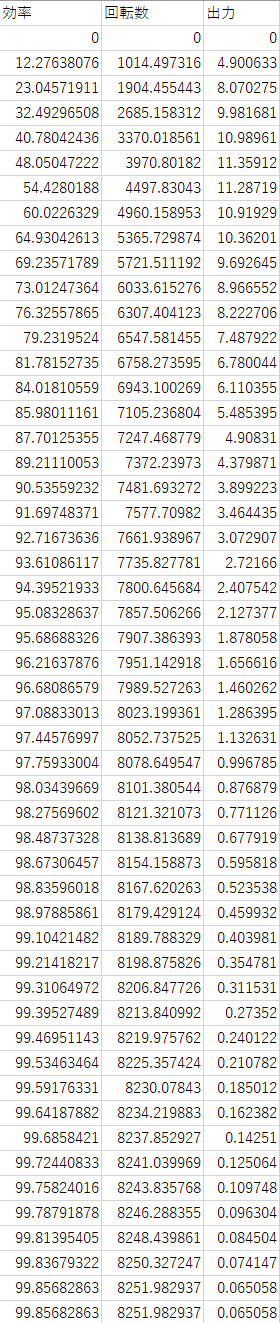
\includegraphics[width=3cm]{./Image/tekiyou_csv_kakunin.png}
%     }
%     \caption{図\ref{fig:tekiyou_csv}から効率と回転数を算出}
% 	\label{fig:kakunin_csv}
% \end{figure}

\subsubsection{定格電圧}
図\ref{fig:tekiyou_mortoku}の特性表にある定格電圧の値と、
図\ref{fig:tekiyou_csv_wakariyasui}のsignalVoltage1.p.vが持つ値の中で、先頭にある値が同値である。
したがって、正しく出力していることが確認できる。

\subsubsection{始動電流}
図\ref{fig:tekiyou_mortoku}の特性表にある始動電流の値と、
図\ref{fig:tekiyou_csv_wakariyasui}のsignalVoltage1.n.iが持つ値の中の最大値が同値である。
したがって、正しく出力していることが確認できる。

\subsubsection{停動トルク}
図\ref{fig:tekiyou_mortoku}の特性表にある停動トルクの値と、
図\ref{fig:tekiyou_csv_wakariyasui}のinertia1.flange\_a.tauが持つ値の中の最大値が同値である。
したがって、正しく出力していることが確認できる。

\subsubsection{最大効率}
図\ref{fig:tekiyou_mortoku}の特性表にある最大効率の値と、
図\ref{fig:tekiyou_csv_wakariyasui}の効率が持つ値の中の最大値が同値である。
したがって、正しく出力していることが確認できる。

\subsubsection{定格トルク}
図\ref{fig:tekiyou_mortoku}の特性表にある定格トルクの値と、
図\ref{fig:tekiyou_csv_wakariyasui}のinertia1.flange\_a.tauが持つ値の中の、最大効率を出した時の値が同値である。
したがって、正しく出力していることが確認できる。

\subsubsection{定格回転数}
図\ref{fig:tekiyou_mortoku}の特性表にある定格回転数の値と、
図\ref{fig:tekiyou_csv_wakariyasui}の回転数が持つ値の中の、最大効率を出した時の値が同値である。
したがって、正しく出力していることが確認できる。

\subsubsection{定格電流}
図\ref{fig:tekiyou_mortoku}の特性表にある定格電流と、
図\ref{fig:tekiyou_csv_wakariyasui}のsignalVoltage1.n.iが持つ値の中の、
最大効率を出した時の値が同値である。
したがって、正しく出力していることが確認できる。

\subsubsection{定格出力}
% 出力は、\mbox{ トルク $(\mathrm{N \cdot m})$} $\times$ \mbox{角速度 $(\mathrm{rad/s})$} で算出することが可能である。
図\ref{fig:tekiyou_mortoku}の特性表にある定格出力と、
図\ref{fig:tekiyou_csv_wakariyasui}の出力が持つ値の中の、最大効率を出した時の値が同地である。
したがって、正しく出力していることが確認できる。

% 図\ref{fig:tekiyou_mortoku}の特性表にある出力と、図\ref{fig:tekiyou_csv}の最大効率時のinertia1.flange\_a.tauが持つ値と、inertia1.flange\_a.wが持つ値を(\ref{siki:speed})式に適用した結果が同値である。
% よって、正しく出力していることが確認できる。
\subsubsection{最大回転数}
図\ref{fig:tekiyou_mortoku}の特性表にある最大回転数と、
図\ref{fig:tekiyou_csv_wakariyasui}の回転数が持つ値の中の最大値が同値である。
したがって、正しく出力していることが確認できる。

\subsection{特性グラフの確認}
出力した特性グラフが正しく算出できているか確認した結果を、以下に示す。

\subsubsection{「トルク $\times$ 電流」グラフ}
図\ref{fig:tekiyou_mortoku}の特性グラフにある「トルク $\times$ 電流」グラフに、
図\ref{fig:tekiyou_csv}のinertia1.flange\_a.tauの持つ値と、
signalVoltage1.n.iが持つ値が存在するので、正しく生成していることが確認できる。

\subsubsection{「トルク $\times$ 回転数」グラフ}
図\ref{fig:tekiyou_mortoku}の特性グラフにある「トルク $\times$ 回転数」グラフに、
図\ref{fig:tekiyou_csv}のinertia1.flange\_a.tauの持つ値と、
回転数が持つ値が存在するので、正しく生成していることが確認できる。

\subsubsection{「トルク $\times$ 効率」グラフ}
図\ref{fig:tekiyou_mortoku}の特性グラフにある「トルク $\times$ 効率」グラフに、
図\ref{fig:tekiyou_csv}のinertia1.flange\_a.tauの持つ値と、
効率が持つ値が存在するので、正しく生成していることが確認できる。

\subsubsection{「トルク $\times$ 出力」グラフ}
図\ref{fig:tekiyou_mortoku}の特性グラフにある「トルク $\times$ 出力」グラフに、
図\ref{fig:tekiyou_csv}のinertia1.flange\_a.tauの持つ値と、
出力が持つ値が存在するので、正しく生成していることが確認できる。


\section{ブラシ付きDCモータのModelicaモデルをサブシステムとするモデル}
今回適用するブラシ付きDCモータのModelicaモデルをサブシステムとするモデルは、
図\ref{fig:tekiyou_tanntai}のモデルと同じ性能になるよう設計しており、
どちらのモータ特性表も同じ内容になっていることを確認する。

今回適用するブラシ付きDCモータのModelicaモデルをサブシステムとするモデルを、
図\ref{fig:tekiyou_sub}に、生成したモータ特性表を図\ref{fig:sub_mortoku}にそれぞれ示す。

\begin{figure}[t]
	\centering
	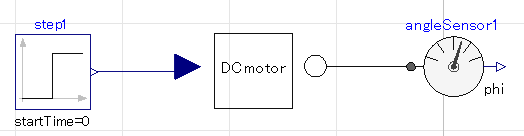
\includegraphics[width=10cm]{./Image/tekiyou_sub.png}
	\caption{適用するブラシ付きDCモータのModelicaモデルをサブシステムとするモデル}
	\label{fig:tekiyou_sub}
\end{figure}

\begin{figure}[t]
	\centering
	\fbox{
	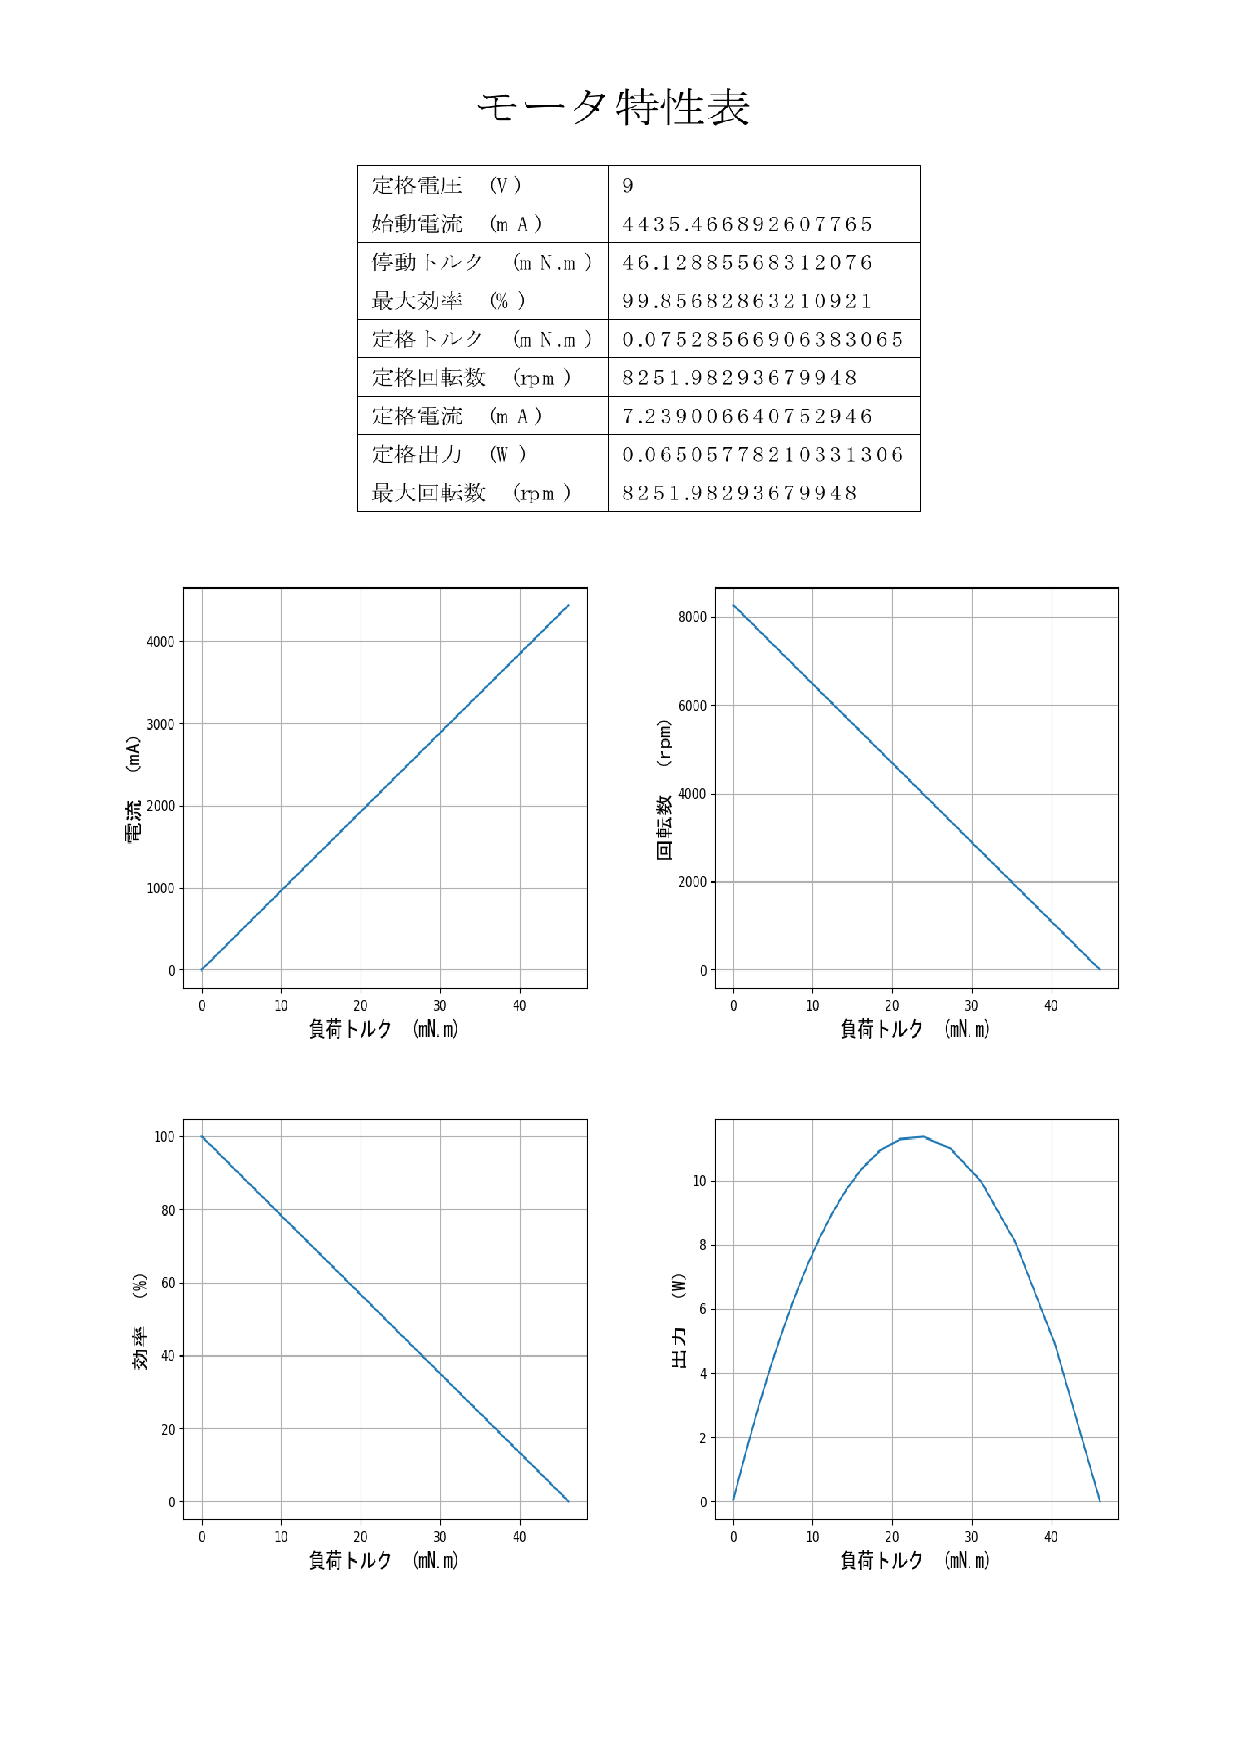
\includegraphics[width=16cm,pagebox=cropbox]{Image/characteristicTable_kakunin.pdf}
	}
	\caption{図\ref{fig:tekiyou_sub}のモータ特性表}
	\label{fig:sub_mortoku}
\end{figure}

図\ref{fig:tekiyou_mortoku}と図\ref{fig:sub_mortoku}の内容が同じであるため、2つのモデルから生成したモータ特性表の各要素が、同値になっていることが確認できる。

\todo{おわりにで書く:『よって、モータ特性表自動生成ツールは、「ブラシ付きDCモータのModelicaモデル」と「ブラシ付きDCモータのModelicaモデルをサブシステムとするモデル」に対応していることが確認できる。』}
